\section{Precision of Indoor Location}\label{sec:estimoteprecision}
Another core part of our system is indoor location. 
For the ``point-to-select'' part of our system to work as intended, 
we need high indoor precision. 
In \Cref{sec:designindoorlocation} we mentioned that Estimote claims the accuracy to be \num{0.5}-\num{1} meters.
In this section we test if that is actually the case, 
or even if we can achieve better results than that. 
This section will contain some of the measurements from our tests. 
All of the measurements can be found in \Cref{app:estimotetestresults}

We test this by comparing the position we get from the application, 
to the actual position we have in the room. 
We test in with the \num{4} settings from \Cref{table:rooms}.

\begin{table}
    \centering
    \begin{tabular}{l| l c c}
        Name & Size in meters & \# of Beacons & \# of Tests\\ \hline
        Room 1 & $5 \times 5$ & 4 & 8 \\
        Room 2 & $8 \times 8$ & 4 & 7 \\
        Room 3 & $17.9 \times 17.9$ & 4 & 3 \\
        Room 4 & $4.9 \times 9.95$ & 4/8 &  33
    \end{tabular}
    \caption{Room settings}
    \label{table:rooms}
\end{table}

We test in different settings to measure if, and how much, 
the size of the room matters in terms of accuracy. 
We decided to test outside in an area where there were none or few WiFi signals,
as WiFi shares the same same radio frequency as BLE (\SI{2.4}{\GHz}). 
We have performed tests both with and without movement. 
The same person have used to perform all the movement tests. 

\subsection{Setup}\label{sec:setup}
Room 1 and Room 2 were setup in an auditorium. 
We used tables to simulate walls, 
and we placed the beacons on chairs on top of the tables. 
The setup can be seen in \Cref{fig:audtest} and illustrated in \Cref{fig:precisiontest:illustration}. 
\todo[author=Thalley]{Insert number of 2.4 GHz access points}
\begin{figure}[!htb]
    \centering
    \includegraphics[width=\textwidth]{drawings/audtest}
    \caption{The setup for Room 1 and Room 2. Room 1 is marked as the inner (blue) square and is $5 \times 5$ meters. Room 2 is marked as the outer (red) square and is $8 \times 8$ meters. The Estimote beacons are placed on the chairs.}
    \label{fig:audtest}
\end{figure}

\begin{figure}[!htb]
    \centering
    \input{drawings/audtestillustration.tikz}
    \caption{Illustration of room used for indoor location precision test. The full (blue) circles represent beacons, the dotted line is the walking path (movement test) and the dotted center circle is the location of the phone (stationary test).}
    \label{fig:precisiontest:illustration}
\end{figure}

The setup consisted of four beacons, one on each wall, 
each using the recommended settings from Estimote \cite{estimote:settings}:
\begin{description}
    \item[Broadcasting Power]{4 dBm}
    \item[Advertising Interval]{200 ms}
    \item[Smart Power Mode]{Enabled}
    \item[Basic Power Mode]{Disabled}
\end{description}

For Room 3, the outdoor ``room'',
we attached the beacons to lampposts. 
We tested outside to see if the number of access points would have, and how much of, 
an impact on the accuracy. 
The ``room'' is illustrated in \Cref{fig:outdoortest}. 
The beacons in this room are slightly off-center (\SI{0.45}{\meter}), 
as we had to use the lampposts' locations. 

\begin{figure}[!htb]
    \centering
    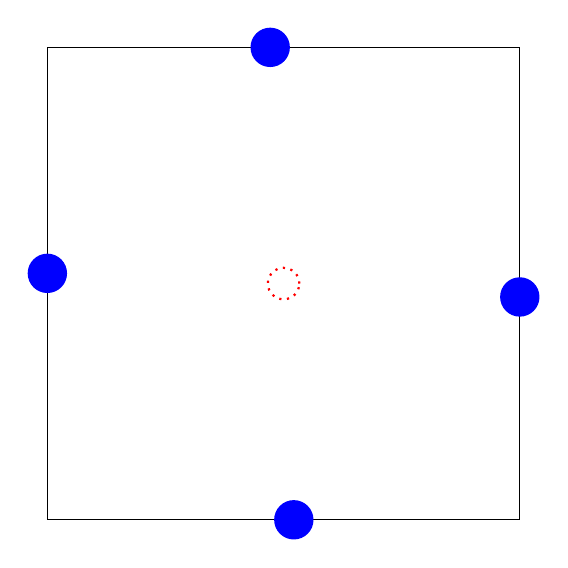
\begin{tikzpicture}

\draw (0,0) rectangle (6,6); % Outline of room
%
\draw[red,thick,dotted] (3,3) circle (0.2); % Phone location

\fill[blue!100!] (3.13, 0) circle (0.25); % Beacon location - Bottom
\fill[blue!100!] (6, 2.83) circle (0.25); % Beacon location - Right
\fill[blue!100!] (2.83, 6) circle (0.25); % Beacon location - Top
\fill[blue!100!] (0, 3.13) circle (0.25); % Beacon location - Left

\end{tikzpicture}
    \caption{Illustration of room used for Estimote accuracy outdoors, with little to no interference from WiFi access points. The full (blue) circles represent beacons, and the dotted center circle is the location of the phone (stationary test).}
    \label{fig:outdoortest}
\end{figure}

Room 4 is a seminar room. 
The setup for Room 4 for the stationary tests,
were exactly the same as the Room 1 and 2. 
We also did movement tests in this room, 
where the user walked around near the walls as with Room 1 and 2. 
We did, however, also test movement where the user walked in a \emph{bowtie},
illustrated by \Cref{fig:bowtie4beacons}. 
We did this to see if we it would have any effect if we did not walk near the beacons all the time. 
We also tried to perform tests with \num{8} beacons in this room, 
illustrated by \Cref{fig:bowtie8beacons}. 

\begin{figure}[!htb]
    \begin{minipage}[b]{0.45\textwidth}
      \centering
        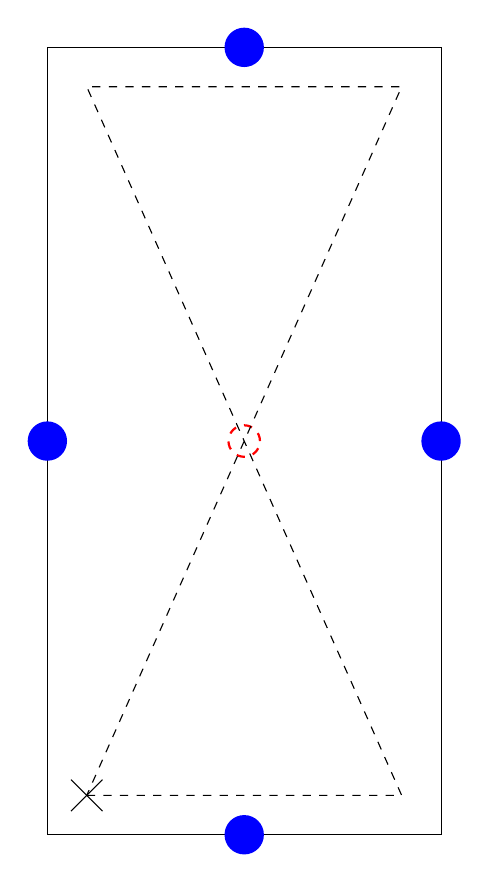
\begin{tikzpicture}

\draw (0,0) rectangle (5,10); % Outline of room

\draw[red,thick,dashed] (2.5,5) circle (0.2); % Phone location

\fill[blue!100!] (2.5, 0) circle (0.25); % Beacon location - Bottom
\fill[blue!100!] (5, 5) circle (0.25); % Beacon location - Right
\fill[blue!100!] (2.5, 10) circle (0.25); % Beacon location - Top
\fill[blue!100!] (0, 5) circle (0.25); % Beacon location - Left

% Walking path
\draw[dashed] (0.5,0.5) -- (4.5,0.5) -- (0.5, 9.5) -- (4.5, 9.5) -- cycle;

% Start / stop point of walking path
\draw (0.3,0.7) -- (0.7,0.3);
\draw (0.3,0.3) -- (0.7,0.7);

\end{tikzpicture}
        \caption{Room 4 bowtie setup using four beacons.}
        \label{fig:bowtie4beacons}
    \end{minipage}
    \hfill
    \begin{minipage}[b]{0.45\textwidth}
      \centering
        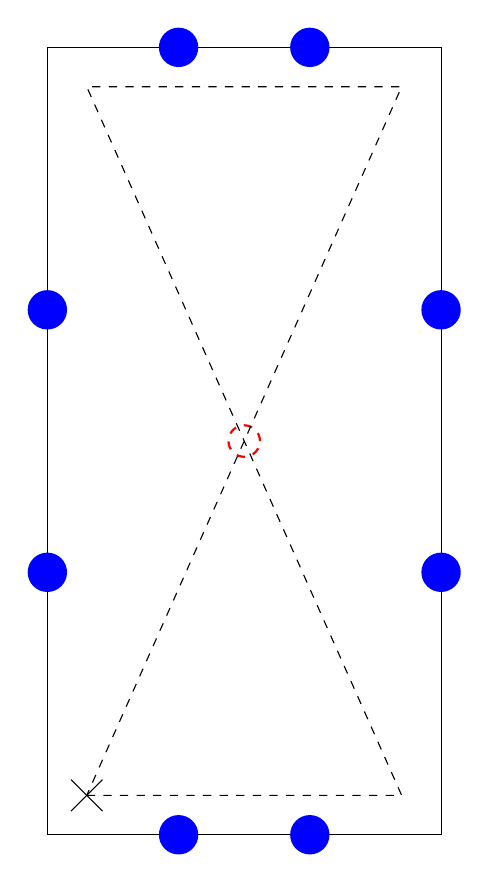
\begin{tikzpicture}

\draw (0,0) rectangle (5,10); % Outline of room

\draw[red,thick,dashed] (2.5,5) circle (0.2); % Phone location

\fill[blue!100!] (1.6667, 0) circle (0.25); % Beacon location - Bottom Left
\fill[blue!100!] (3.3334, 0) circle (0.25); % Beacon location - Bottom Right
\fill[blue!100!] (5, 6.6666) circle (0.25); % Beacon location - Right Top
\fill[blue!100!] (5, 3.3333) circle (0.25); % Beacon location - Right Bottom
\fill[blue!100!] (1.6667, 10) circle (0.25); % Beacon location - Top Left
\fill[blue!100!] (3.3334, 10) circle (0.25); % Beacon location - Top Right
\fill[blue!100!] (0, 6.6666) circle (0.25); % Beacon location - Left Top
\fill[blue!100!] (0, 3.3333) circle (0.25); % Beacon location - Left Bottom


% Walking path
\draw[dashed] (0.5,0.5) -- (4.5,0.5) -- (0.5, 9.5) -- (4.5, 9.5) -- cycle;

% Start / stop point of walking path
\draw (0.3,0.7) -- (0.7,0.3);
\draw (0.3,0.3) -- (0.7,0.7);

\end{tikzpicture}
        \caption{Room 4 bowtie setup using eight beacons.}
        \label{fig:bowtie8beacons}
    \end{minipage}
\end{figure}

\Cref{table:precisiontest:roomsize} shows the test setups from these rooms,
using the recommended settings.
In \Cref{sec:settings}, we change some of the settings to determine if they have any effect.

\begin{table}[!htb]
    \centering
    \begin{tabular}{l| l l c c}
        Room   & Phone Position & Duration 	       & Count & \# of Beacons \\ \hline
        Room 1 & Center         & \SI{1}{\minute}  & 4  & 4 \\ 
        Room 1 & Center         & \SI{2}{\minute}  & 1     & 4 \\ 
        Room 1 & Moving         & NA               & 3     & 4 \\
        Room 2 & Center         & \SI{1}{\minute}  & 3     & 4 \\ 
        Room 2 & Center         & \SI{2}{\minute}  & 1     & 4 \\
        Room 2 & Moving         & NA               & 3     & 4 \\ 
        Room 3 & Center         & \SI{1}{\minute}  & 3     & 4 \\ 
        Room 4 & Center         & \SI{1}{\minute}  & 3     & 4 \\ 
        Room 4 & Center         & \SI{1}{\minute}  & 3     & 8 \\ 
        Room 4 & Moving         & NA       & 3     & 4 \\
        Room 4 & Moving         & NA       & 3     & 8 \\
        Room 4 & Moving-Bowtie  & NA       & 3     & 4 \\
        Room 4 & Moving-Bowtie  & NA       & 3     & 8 \\
    \end{tabular}
    \caption{Tests conducted with varying room size and recommended beacon configuration.}
    \label{table:precisiontest:roomsize}
\end{table}


\subsection{Stationary Accuracy}
This section contains the results from measuring the accuracy of the tests, 
where we have placed a phone and logged the locations. 
\Cref{fig:room3:1:4:c,fig:room4:1:4:c,fig:room4:1:4:2.8,fig:room4:1:8:c} shows selected results as heatmaps. 
In these heatmaps, the heat, or intensity, 
shows the number of coordinates measured at that coordinate. 

%HEATMAPS
\begin{figure}[!htb]
  \begin{minipage}[t]{0.48\textwidth}
    \includegraphics[width=\textwidth]{\heatmap{32}}
    \caption{Room 3, \SI{1}{\minute}, 4 beacons, centered}
    \label{fig:room3:1:4:c}
  \end{minipage}\hfill
  \begin{minipage}[t]{0.48\textwidth}
    \includegraphics[width=\textwidth]{\heatmap{36}}
    \caption{Room 4, \SI{1}{\minute}, 4 beacons, centered}
    \label{fig:room4:1:4:c}
  \end{minipage}
\end{figure}

\begin{figure}[!htb]
  \begin{minipage}{0.48\textwidth}
    \includegraphics[width=\textwidth]{\heatmap{43}}
    \caption{Room 4, \SI{1}{\minute}, 4 beacons, at (2,8)}
    \label{fig:room4:1:4:2.8}
  \end{minipage}\hfill
  \begin{minipage}{0.48\textwidth}
    \includegraphics[width=\textwidth]{\heatmap{51}}
    \caption{Room 4, \SI{1}{\minute}, 8 beacons, centered}
    \label{fig:room4:1:8:c}
  \end{minipage}
\end{figure}

The heatmaps shows that none of the results are very accurate. 
However, we do see some consistency in the data, in the form of clusters. 
This is primary seen in \Cref{fig:room3:1:4:c,fig:room4:1:4:2.8}. 
We do see some clustering in \Cref{fig:room4:1:4:c}. 
We expect the reason why the data is spread out like that, 
is a combination of the fact that the phone is centered, \ie not near any beacons,
and that we are near WiFi access points with the same frequency. 
We see a similar tendency in in \Cref{fig:room4:1:8:c}, 
but we expect that the increased spreading here is due to interference from using more beacons. 

%MEAN ERROR
Since we know the location of the phone, 
we can measure the distance error of each coordinate we get from Estimote. 
\todo[author=Thalley]{Insert distance error and mean distance error}

\subsection{Moving Accuracy}
In this section we measure the accuracy of the Estimote beacons,
while the phone is in motion. 
We walk around in a given path, 
as described by \Cref{sec:setup}.
\Cref{fig:room1:4:m,fig:room2:4:m,fig:room4:4:m} shows selected heatmaps of walking near the walls, 
where \Cref{fig:room4:4:b,fig:room4:8:b} shows selected heatmaps of walking in a bowtie pattern.
%HEATMAPS
\begin{figure}[!htb]
  \begin{minipage}{0.48\textwidth}
    \includegraphics[width=\textwidth]{\heatmap{08}}
    \caption{Room 1, 4 beacons, moving}
    \label{fig:room1:4:m}
  \end{minipage}\hfill
  \begin{minipage}{0.48\textwidth}
    \includegraphics[width=\textwidth]{\heatmap{14}}
    \caption{Room 2, 4 beacons, moving}
    \label{fig:room2:4:m}
  \end{minipage}
\end{figure}
\begin{figure}[!htb]
  \centering
  \includegraphics[width=0.48\textwidth]{\heatmap{37}}
  \caption{Room 4, 4 beacons, moving}
  \label{fig:room4:4:m}
\end{figure}

\Cref{fig:room1:4:m,fig:room2:4:m} shows that the coordinates we get, 
were relatively close to where we walked, 
but had trouble near the corners, \ie further away from the beacons. 
\Cref{fig:room4:4:m} shows poor results. 
The main difference between rooms 1 and 2 and Room 4,
besides the size,  
is that Room 4 has actual walls, 
instead of the simulated walls. 
As walls can bounce radio waves from the beacons,
this is likely the reason why the results from Room 4 are worse. 

\begin{figure}[!htb]
  \begin{minipage}{0.48\textwidth}
    \includegraphics[width=\textwidth]{\heatmap{40}}
    \caption{Room 4, 4 beacons, bowtie}
    \label{fig:room4:4:b}
  \end{minipage}\hfill
  \begin{minipage}{0.48\textwidth}
    \includegraphics[width=\textwidth]{\heatmap{48}}
    \caption{Room 2, 8 beacons, bowtie}
    \label{fig:room4:8:b}
  \end{minipage}
\end{figure}
Like with \Cref{fig:room4:4:m}, \Cref{fig:room4:4:b,fig:room4:8:b} show poor results. 
This is likely due to walls, as with before, 
but also that we are now spending more time walking further away from beacons, 
than we did in \Cref{fig:room1:4:m,fig:room2:4:m}.

\subsection{Changing Settings}\label{sec:settings}
For this test the objective was to test the accuracy of the location system,
using different settings. 
We use Room 4 with 4 beacons for these tests. 
The tests conducted in this room, 
had the phone placed on a table in the center of the room, 
and logging position data for a duration of one minute.
This was done three times, 
and then the settings of the beacons were changed.

The difference settings we tested are shown in \Cref{table:precisiontest:settings}.

\begin{table}[!htb]
  \centering
  \begin{tabular}{l|l}
    Advertising Interval & Broadcasting Power \\ \hline
    200 ms               & 4 dBm              \\ 
    200 ms               & -20 dBm            \\ 
    200 ms               & -12 dBm            \\ 
    200 ms               & -4 dBm             \\ 
    100 ms               & 4 dBm              \\ 
  \end{tabular}
  \caption{Tests conducted with varying settings on the beacons.}
  \label{table:precisiontest:settings}
\end{table}

\todo[author=Thalley]{Insert results}

\subsection{Precision of Indoor Location Conclusion}
From the results, we can conclude that... \todo[author=Thalley]{Write conclusion of precision test based on results}
